% Basic setup 

A flow configuration that combines the complexities of high density-ratios with the interaction between capillary, viscous and inertial stresses is that of a water droplet falling in air under the influence of gravitational acceleration. The problem is characterized by a combination of Reynolds, Weber and Bond numbers, the definitions of which are as follows : 

\begin{align}
We=\frac{\rho_{\rm air} U^2 d}{\sigma} \quad,\quad Re= \frac{\rho_{\rm air} U d}{\mu_{\rm air}} \quad,\quad Bo=\frac{\left(\rho_{\rm water}-\rho_{\rm air}\right) g d^2 }{\sigma}
\end{align}

\vspace*{0.2cm}

In our particular numerical setup, $We \simeq 3.2 $, $Re \simeq 1455 $ and $Bo \simeq 1.2 $, thus corresponding to that of a $3mm$ diameter raindrop (a relatively large one) falling in air at an approximate terminal velocity of  $8$ m/s (interpolated from empirical data, refer to  \cite{gunn1949terminal}). The parameters in the problem setup are given in Table \ref{raindropprop}, and the schematic diagram given by Fig. \ref{setup}. The droplet is initially placed at the center of a cubic domain (3D), whose side is 4 times the diameter of the drop. 

\vspace*{0.2cm}

% -----
\begin{table}[h!]
\begin{center}
\begin{tabular}{ccccccc}
\hline\hline
$\rho_{\rm air}$ & $\rho_{\rm water}$ & $\mu_{\rm air}$ 
& $\mu_{\rm water}$ & $\sigma$ & $d$ & $g$\\
$\left(kg/m^3\right)$ & $\left(kg/m^3\right)$ & $\left(Pa \, s\right)$ 
& $\left(Pa \,s \right)$ & $\left(N/m\right)$ & $(m)$ & $(m /s^{2})$ \\
\hline
1.2 & $0.9982 \times 10^3$ & $1.98 \times 10^{-5}$ & 
$8.9 \times 10^{-4}$ & $0.0728$ & $3 \times 10^{-3}$ & $9.81$\\
\hline\hline
\end{tabular}
\caption{Parameter values used in the simulation of a falling water droplet in air. \label{raindropprop}}
\end{center}
\end{table}
% -----

\vspace*{0.2cm}

In order to properly reproduce and analyse the dynamics of a relatively large drop (high Reynolds flow) such as in our case, the numerical method has to accurately resolve the thin boundary layers, the interaction of such layers with the capillary forces and finally the non-linear feedback of the complex 3D vortical structures present in the wake behind the droplet. Therefore, our objective behind the demonstration of this particular test case is not to develop a high fidelity model of a raindrop, but rather carry out a stringent evaluation of the robustness of our numerical method compared to methods which are not momentum consistent. For such a low Weber number the capillary forces dominate and the droplet should remain intact, and definitely not undergoe any subsequent atomization. 


% -----
\begin{figure}[h!]
\begin{center}
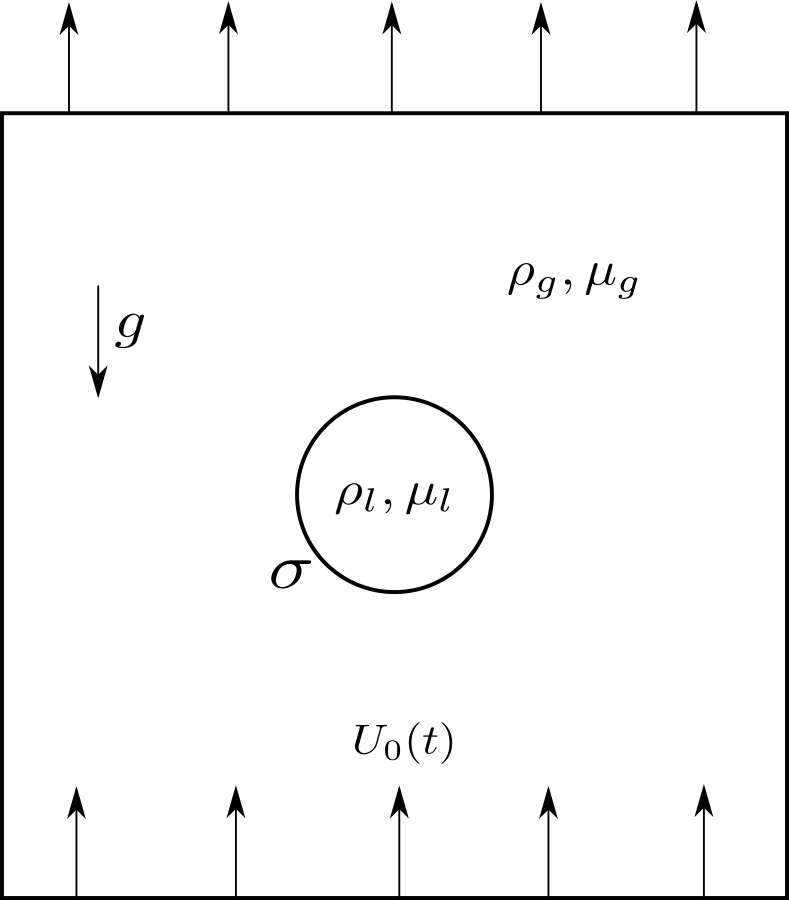
\includegraphics[width=0.5\textwidth]{Figures/Sagar/setup.png}
\end{center}
\caption{A 2D schematic of the numerical setup for the falling raindrop. We apply a uniform inflow velocity condition with $U_0(t)$ and an outflow velocity condition at the top which corresponds to zero gradient of the velocity at the boundary. Boundary conditions on the side walls correspond to those of free slip (no shear stress).}
\label{setup}
\end{figure}
% -----


% -----
\begin{figure}
\begin{center}
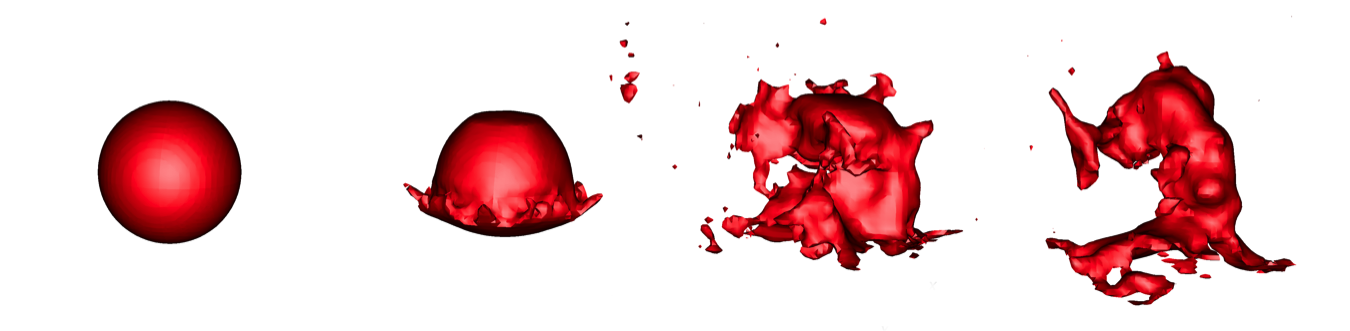
\includegraphics[width=0.75\textwidth]{Figures/cata.png}
\end{center}
\caption{Rain drop test case: catastrophic breakup with non-conserving 
formulation, $D/h=30$.}
\label{cata}
\end{figure}
% -----

Numerical simulations of this test case at moderate resolution (from $D/h=16$ to $D/h=64$) were tested \textit{without} the consistent momentum-conserving scheme described in this paper, results in the catastrophic deformations of the droplet as shown in Fig. \ref{cata}, which we describe as 'fictitious' or 'artificial' atomization as a result of rapidly growing numerical instabilities. This effect was previously uncovered by \cite{Xiao:2014vs} in a similar case involving the sudden interaction of a droplet at rest with a uniform gas flow. The Weber number in that case was also approximately 3, therefore one would expect a nearly spherical droplet shape, but the authors of ref. \cite{Xiao:2014vs} have reported a similar catastrophic deformation. We propose the following explanation in order to account for such numerical artifacts. To start with, we neglect gravity and viscous effects at this relatively large Reynolds number. Also, we are interested in steady-state flow. On the axis and near the hyperbolic stagnation point at the front of the droplet one has $u_2=0$ for the transverse (radial) velocity and for the axial momentum balance

\be
u_1 \partial_1 u_1 = - \frac 1 \rho \partial_1 p.
\nd

Due to the large viscosity and density ratios, it is not possible for the air flow to immediately entrain the water, so the fluid velocity is significantly smaller inside the droplet. In the air the acceleration near the stagnation point is of the order $U^2/D$, whereas the pressure gradient is

\be
\partial_1 p \sim \rho_{a} U^2/D.
\nd
The pressure gradient in the water is much smaller, however in the case of a mixed cell the water density multiplies the air acceleration $U^2/D$, so that
\be
\partial_1 p \sim \rho_{w} U^2/D,
\nd

then a large pressure gradient results in the mixed cell or cells. This large pressure gradient results in a large pressure inside the droplet near the front stagnation point, as shown in Figure \ref{FengXiao}. This large pressure is balanced by surface tension only for a sufficiently large curvature near the droplet front. This explains the presence of a ``dimple'' often observed in low resolution simulations of the falling drop. 

% -----
\begin{figure}
\begin{center}
\begin{tabular}{cc}
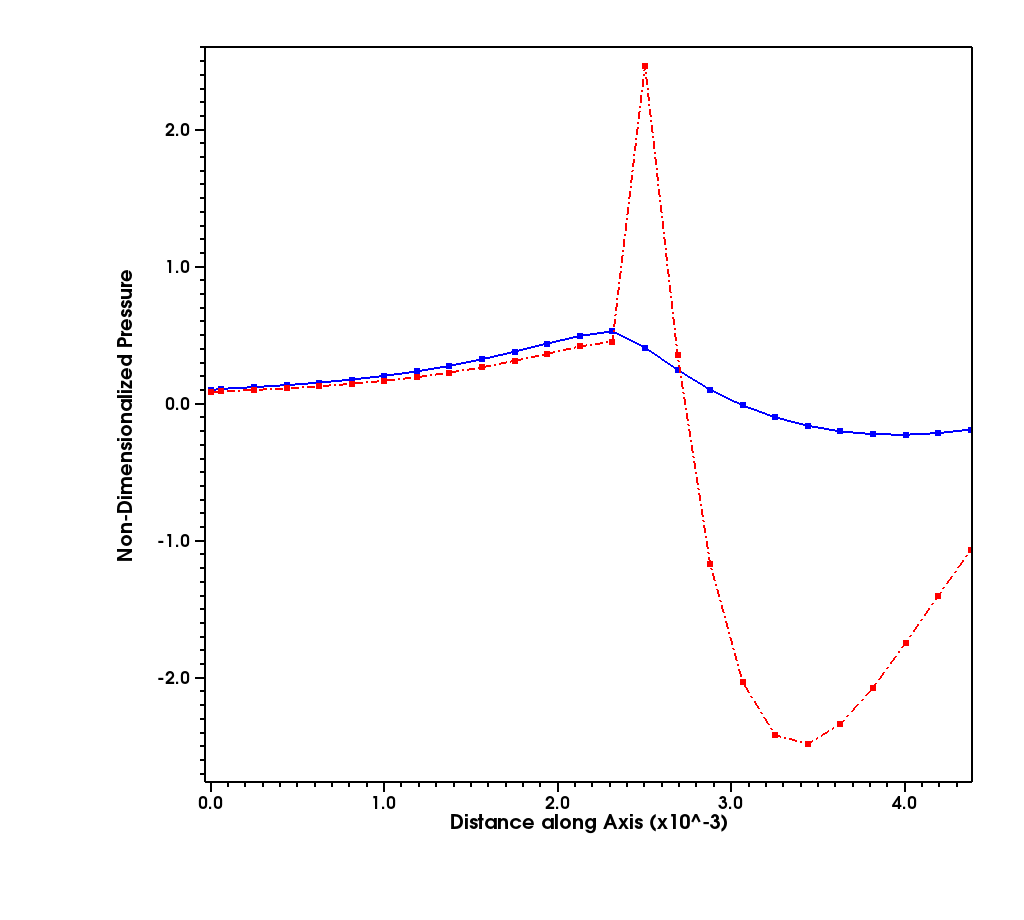
\includegraphics[width=0.45\textwidth]{Figures/Sagar/16ppd_MC_vc_NON-MC.png} &
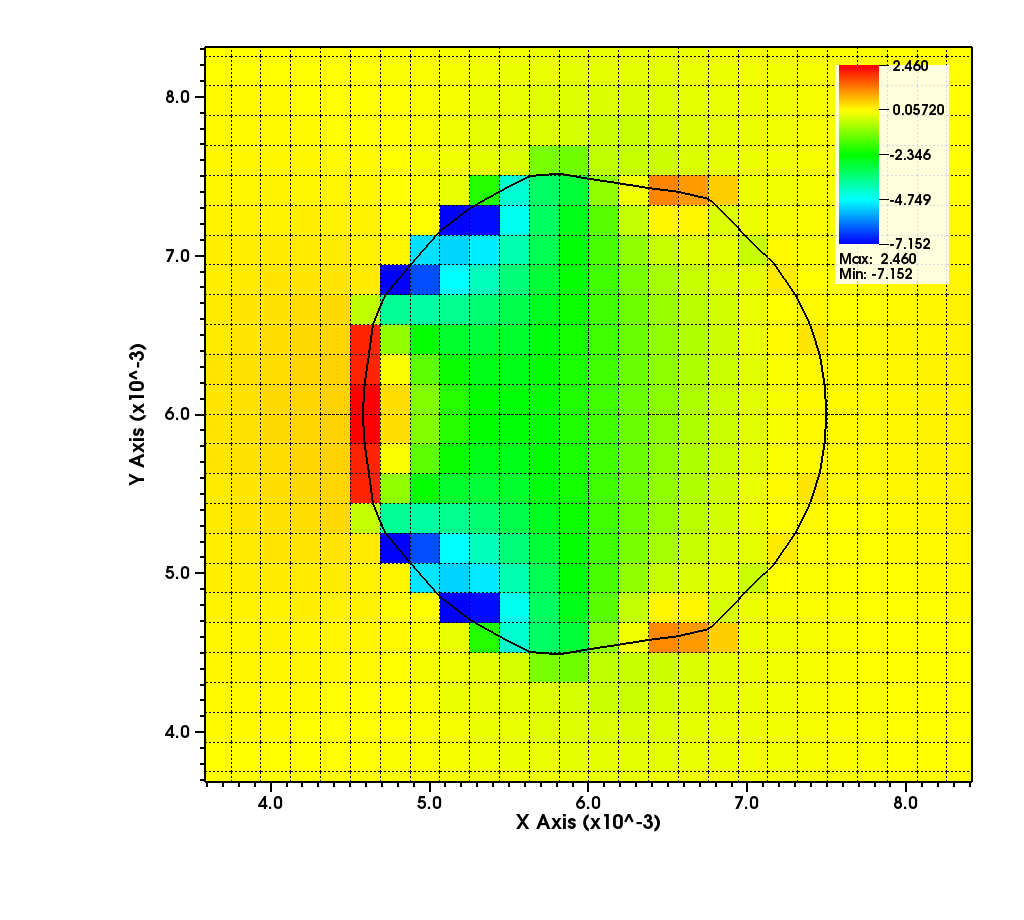
\includegraphics[width=0.45\textwidth]
{Figures/Sagar/non_MC_16ppd_pressure_corrected.png}\\
(a) & (b)
\end{tabular}
\end{center}
\caption{The origin of the pressure peak in the front of the droplet. 
(a) The profile of the pressure on the axis a few timesteps after initialisation 
with the standard, non-momentum conserving method (red) and the present method 
(blue). (b) The pressure distribution immediately after the start of the simulation 
using the standard, non-momentum-conserving method. The pressure peak does
not result yet in the formation of a dimple. In all figures  $D/h = 16$.}
\label{FengXiao}
\end{figure}
% -----

% -----
\begin{figure}
\begin{center}
\begin{tabular}{cc}
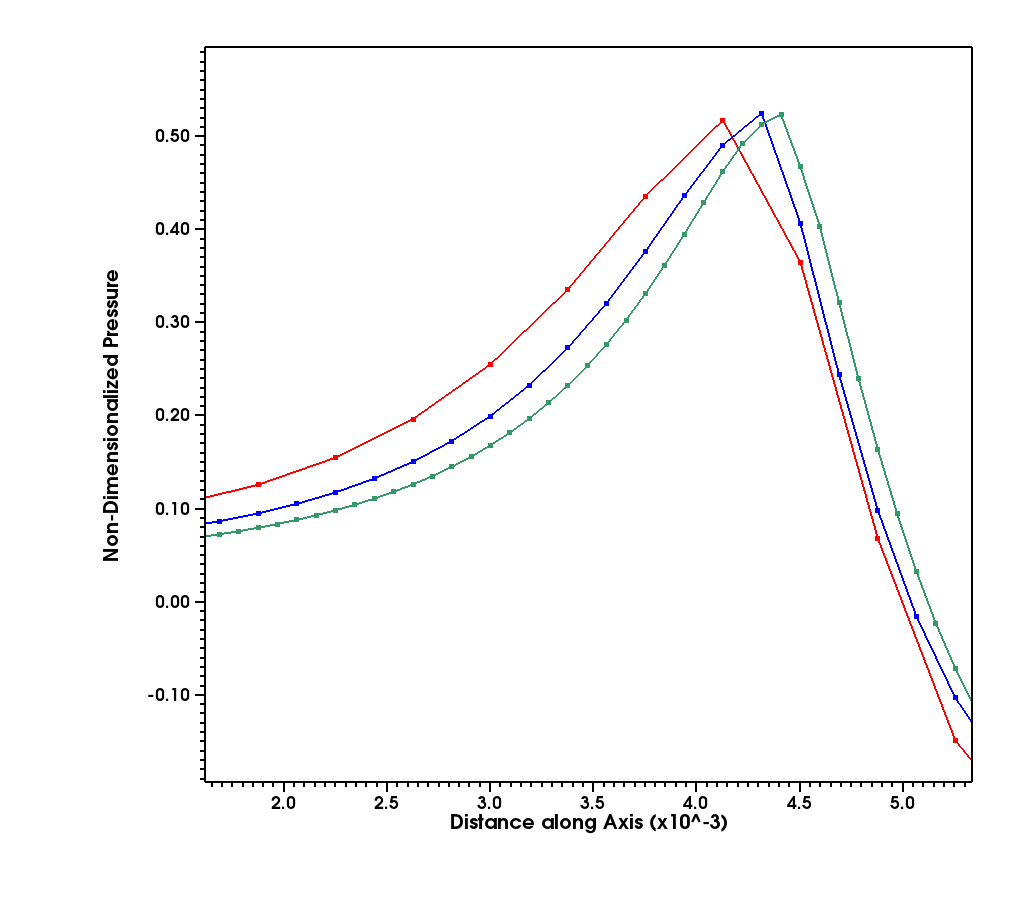
\includegraphics[width=0.45\textwidth]{Figures/Sagar/pressure_rd_MC.png} &
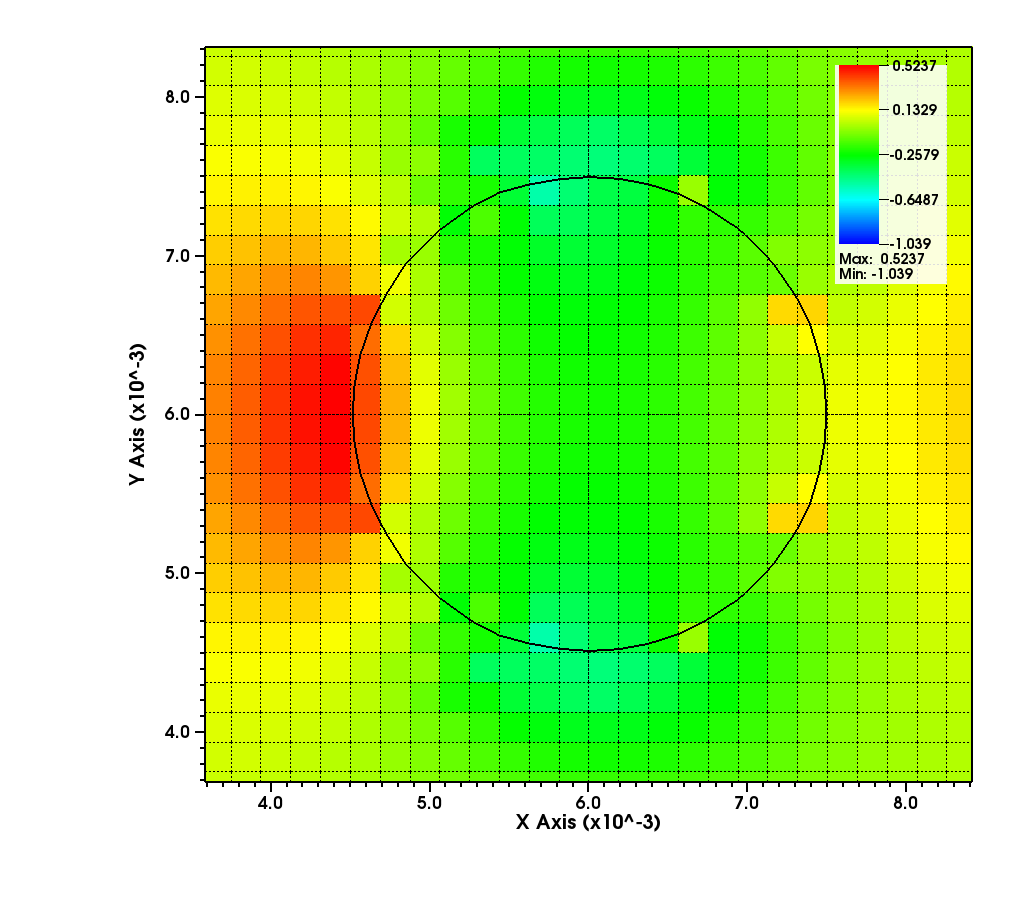
\includegraphics[width=0.45\textwidth]
{Figures/Sagar/16ppd_pressure_corrected.png}\\
(a) & (b)
\end{tabular}
\end{center}
\caption{ (a) The pressure profile on the axis a few timesteps after 
initialisation with the present 
method at various resolutions: $D/h = 8$ (red) , $16$ (blue) and $32$ (green). 
(b) The pressure distribution immediately after the start of the simulation 
using the present method and   $D/h = 16$.}
\label{FengXiao_corrected}
\end{figure}
% -----

\vspace*{0.2cm}

\begin{figure}[!h]
\begin{center}
\begin{tabular}{cc}
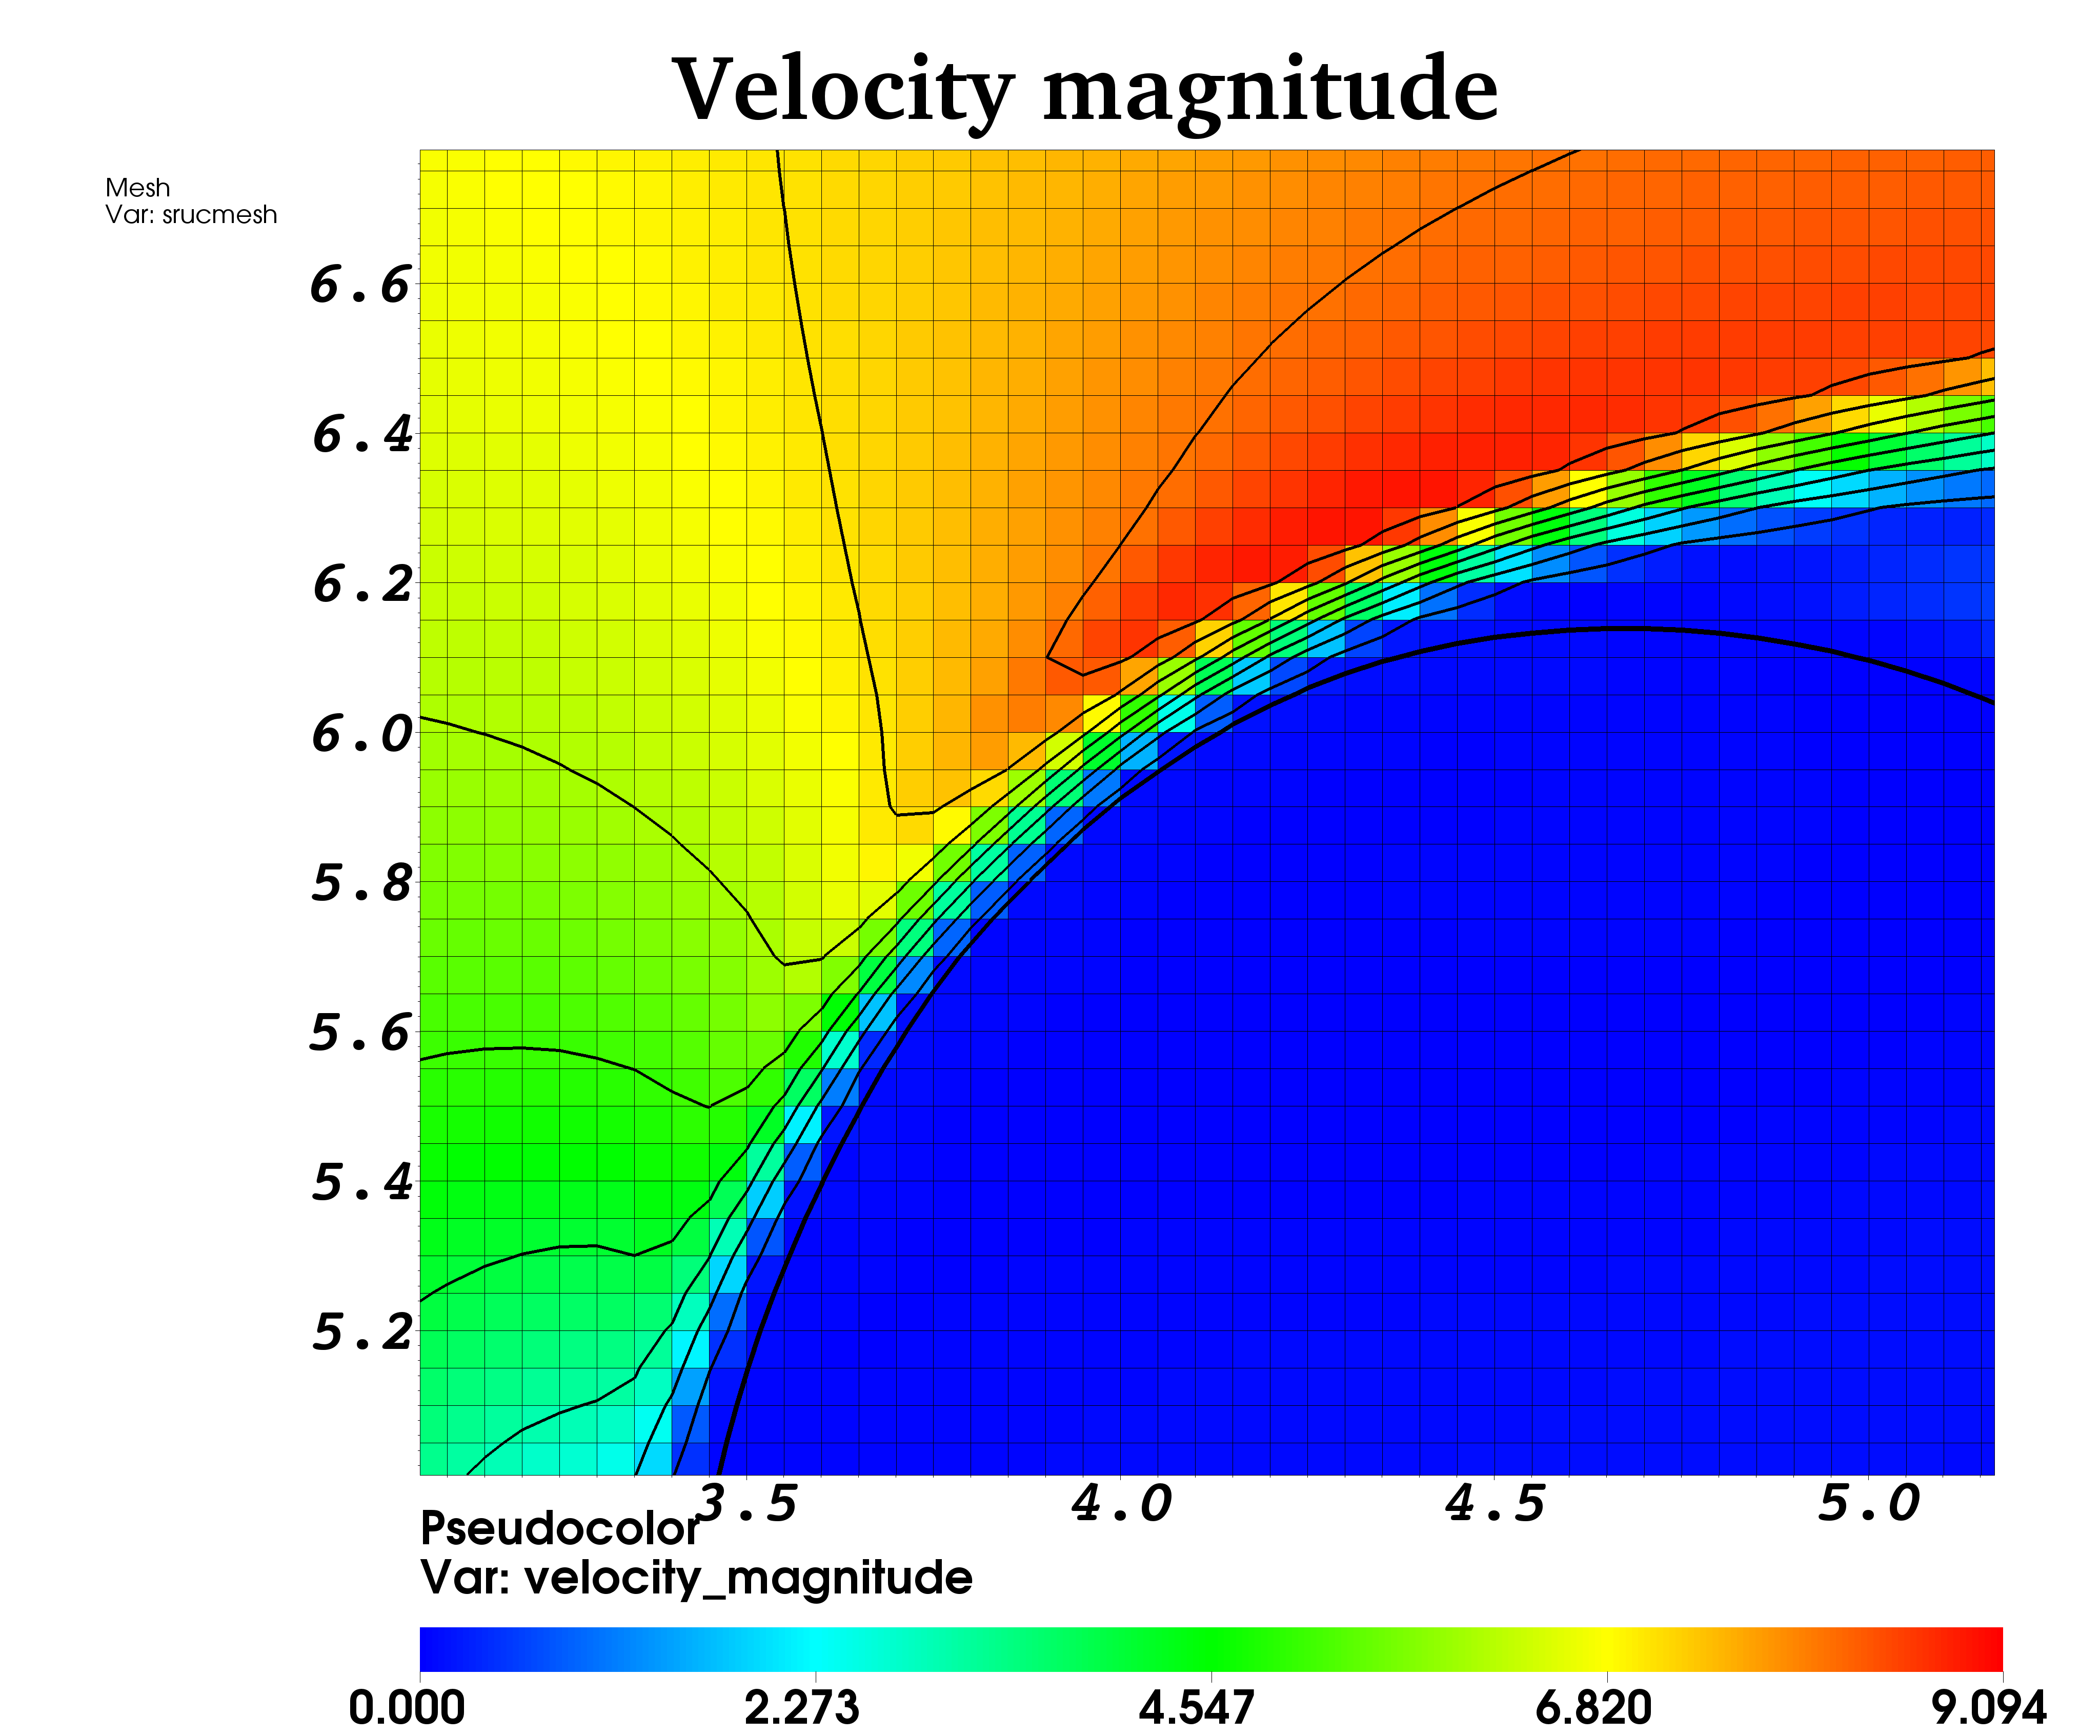
\includegraphics[width=0.42\textwidth]{Figures/vel.png}
& 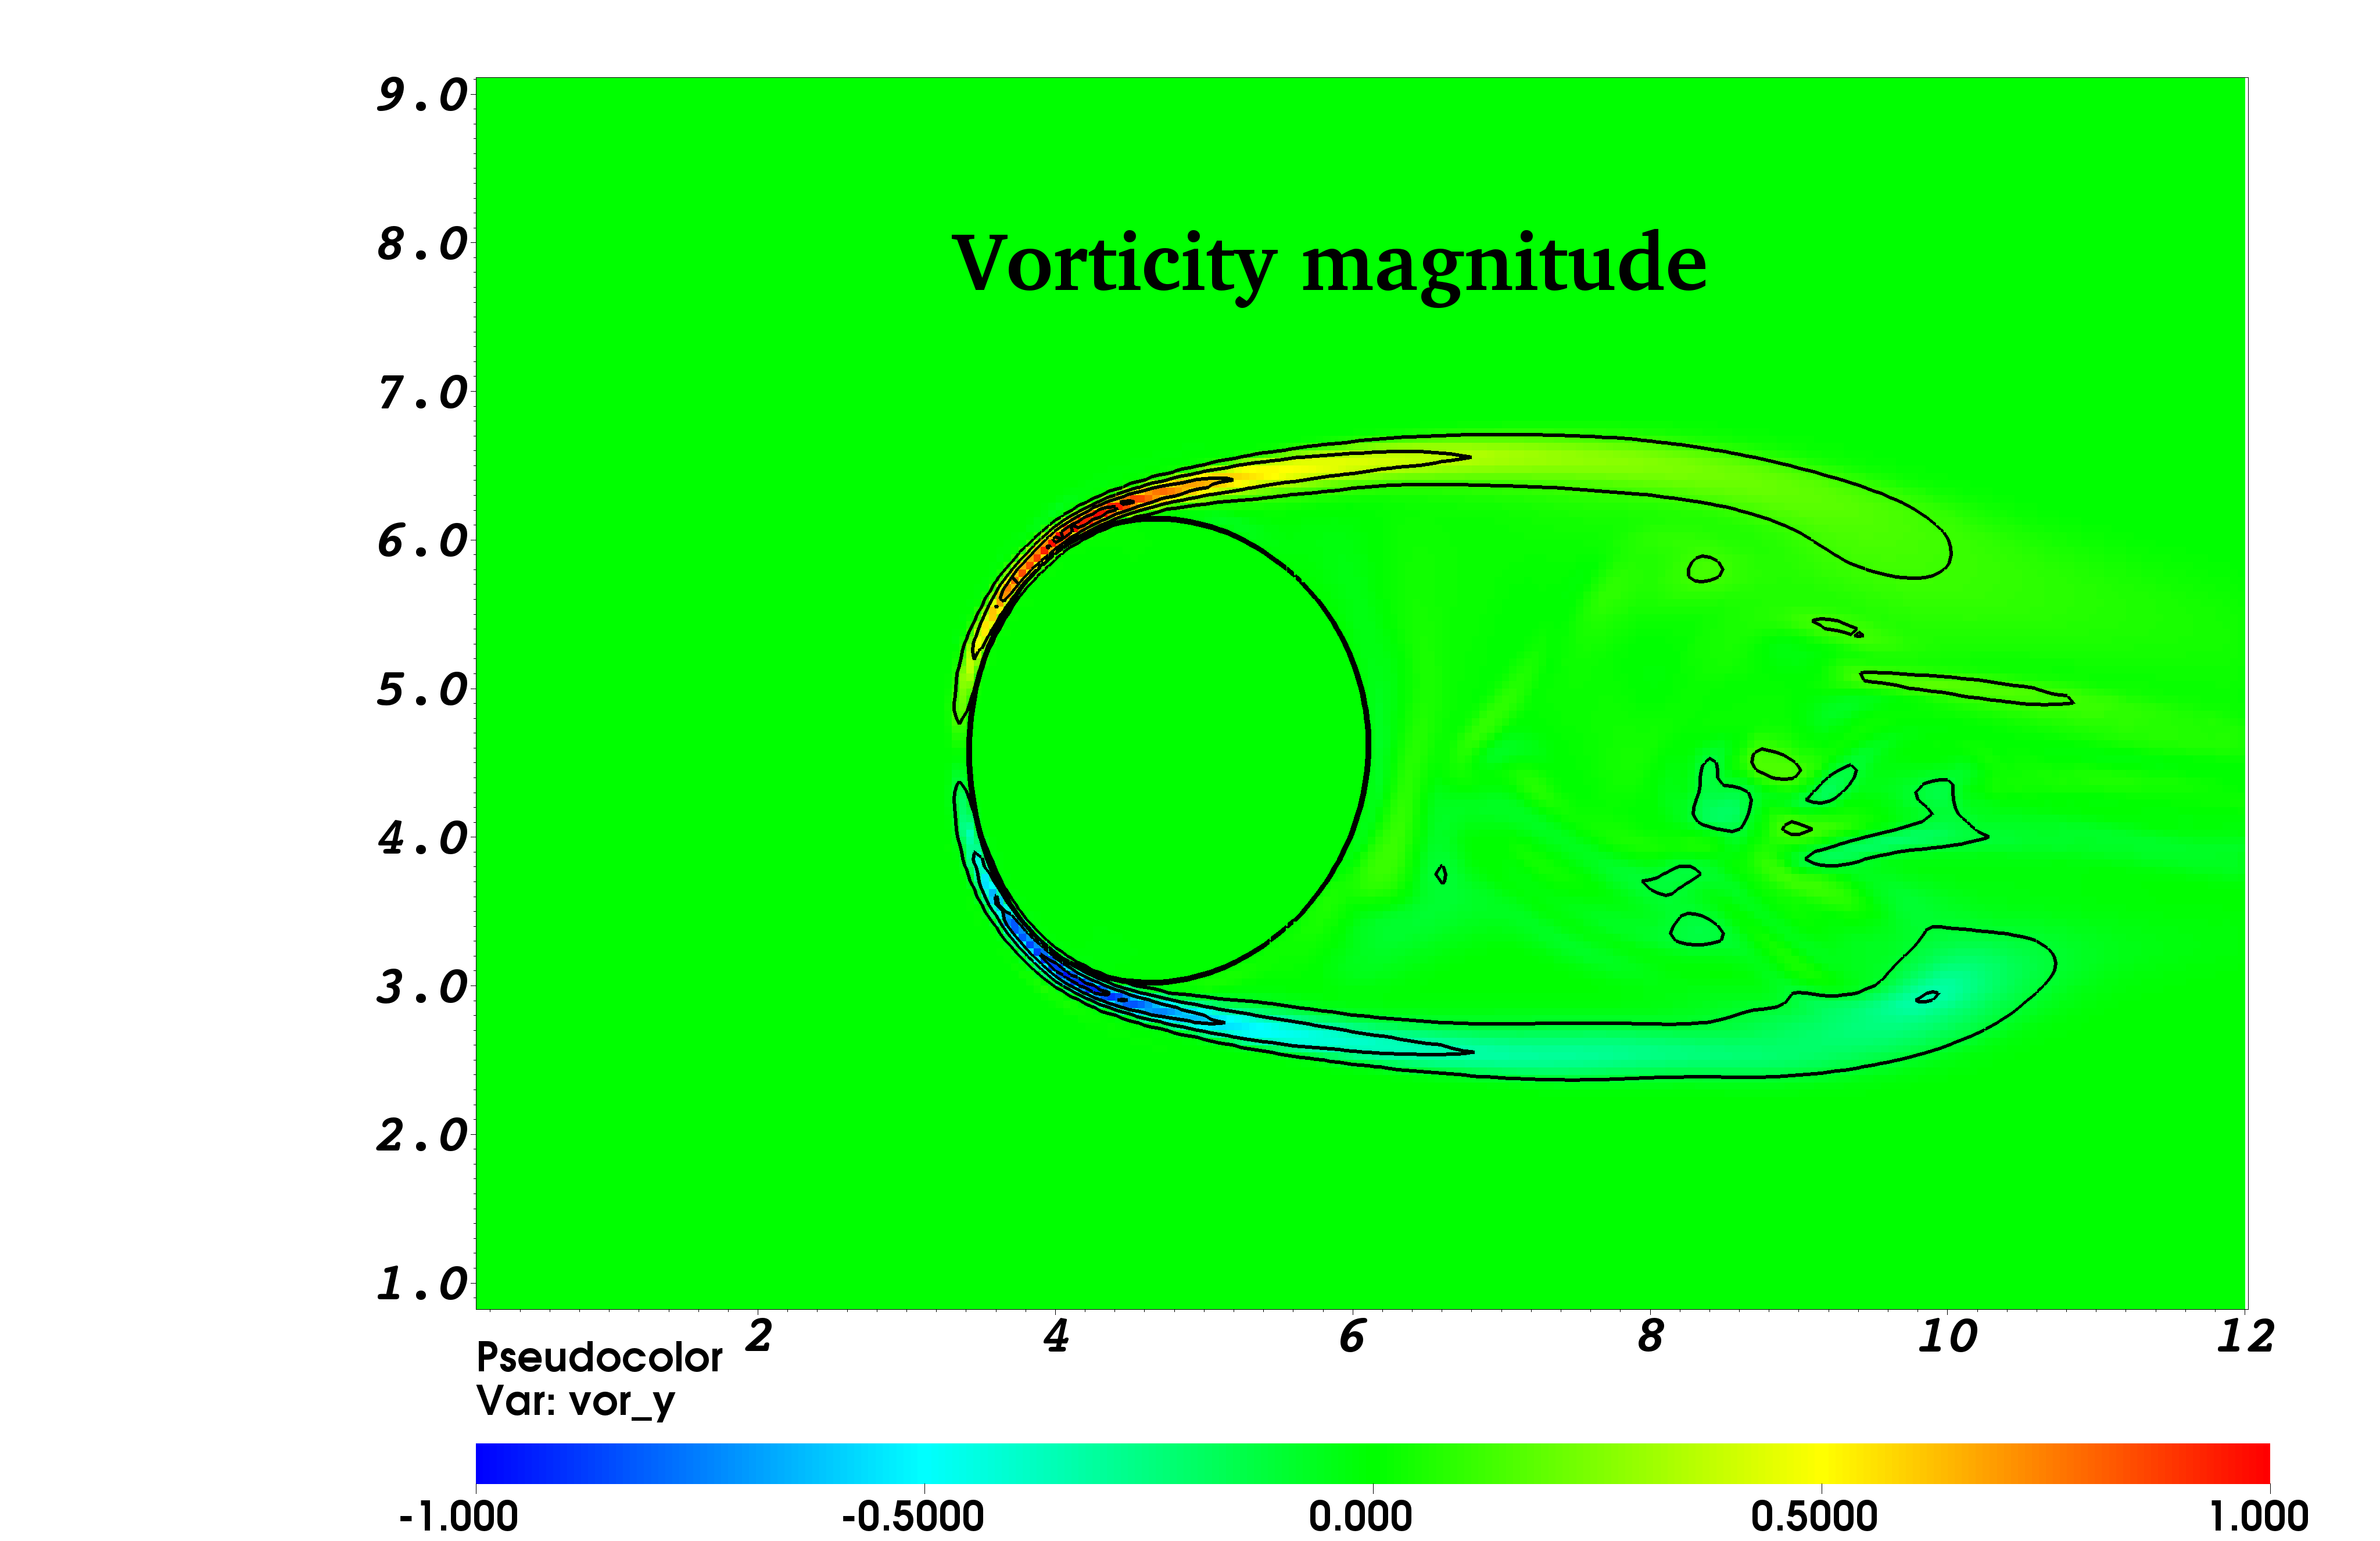
\includegraphics[width=0.48\textwidth]{Figures/vort.png} \\
(a) & (b)
\end{tabular}
\end{center}
\caption{Flow field around the 3 mm droplet with 60 grid points per diameter. 
(a) The velocity magnitude. It is seen that even at this highest resolution 
there are only three points in the boundary layer. (b) The vorticity magnitude. 
The marked separation of the boundary layers is observed with 
a more complex vortical region in the wake.}
\label{magn}
\end{figure}
% -----
\newcommand\DDD{{\cal D}}

Visualization of the flow around the droplets (Figure \ref{magn}) illustrates the challenging nature of the flow configuration, even for such a seemingly simple physical problem. As one can observe, the boundary layers are extremely thin. Therefore, even though the velocity field is continuous across the interface (in the discrete sense) in the absence of mass transfer, there is the appearance of strong velocity variations at the scale of the grid size for such coarse levels of grid refinement. We observe that applying the numerical method described in this paper brings a considerable and systematic improvement over a range of different flux limiters (WENO, ENO, Superbee, QUICK, Verstappen) and CFL numbers, as evidenced by comparing the figures \ref{FengXiao} and \ref{FengXiao_corrected}. 

\vspace*{0.2cm}

\begin{figure}[h!]
\begin{center}
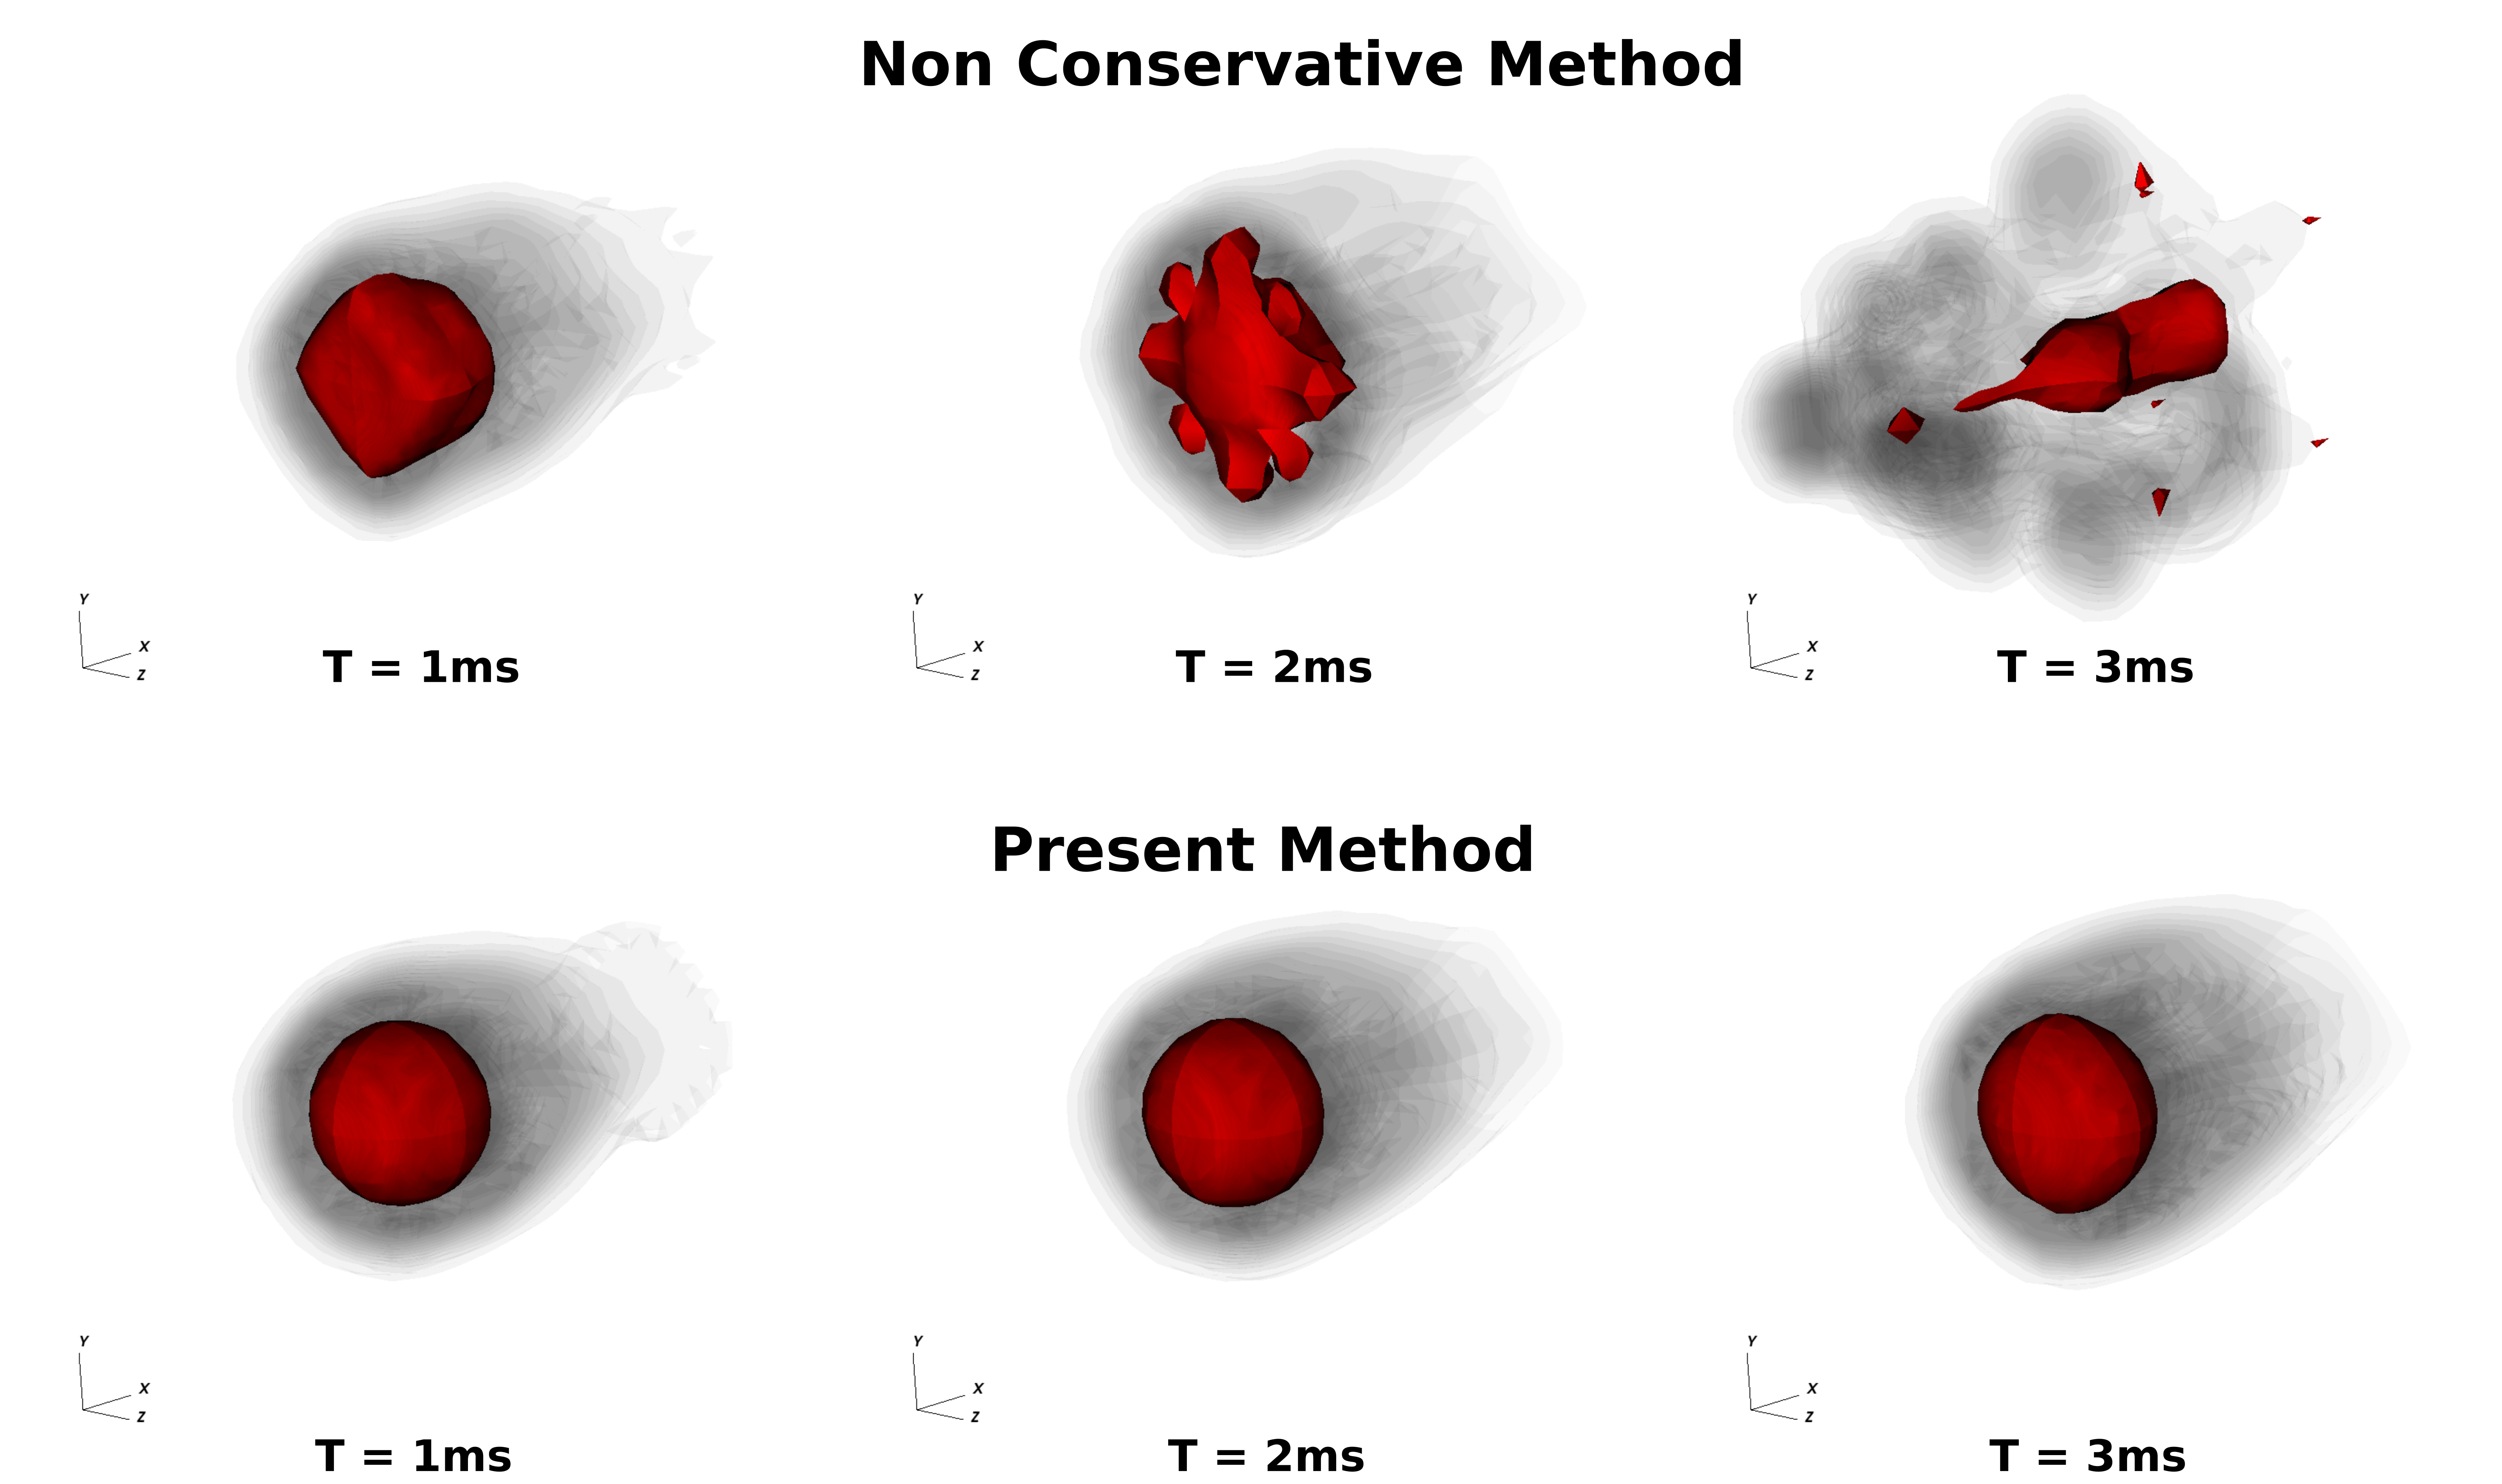
\includegraphics[scale = 0.135]{Figures/Sagar/comparison.png}
\end{center}
\vspace*{-0.5cm}
\caption{A comparison of the temporal evolution between the non conservative version and the present method, using a combination of the WY advection scheme with the QUICK flux limiter. The flow is along the positive X direction, with gravity along the opposite direction. The red contour indicates the isosurface of the volume fraction field corresponding to a value of $0.5$, whereas the black contours surrounding the drop represent isosurfaces of the magnitude of vorticity. The raindrop in the non conservative version displays massive deformations leading to artificial breakup due to rapidly growing numerical instabilities. The droplet resolution for both methods is $D/h = 8$ .}
\label{compare}
\end{figure}

To summarize, the simulations broadly fall into three categories. The first two categories concern those that use the present momentum conserving method, and as a result maintain physical values of the kinetic energy and smooth interfacial shapes. Certain simulations amongst the ones carried out with the present method display some numerical instablities (but not leading to catastrophic deformation) as a function of the choice of advection scheme (CIAM/WY) and flux limiter (QUICK/WENO/ENO/Superbee/Verstappen) combination. Finally, there are simulations carried out without the present method that rapidly blow up, displaying marked peaks or spikes in kinetic energy as a function of time, associated with massively deformed interface shapes (see figure \ref{compare}). Therefore, our studies suggest that certain combinations of the advection scheme and the flux limiter are more numerically robust than others, in particular, the most stable combinations are that of CIAM advection with Superbee limiter and the WY advection with QUICK limiter. As a minor remark, the CIAM advection with the Superbee limiter appear to be quite diffusive. 

\vspace*{0.2cm}

\begin{figure}[h!]
\begin{center}
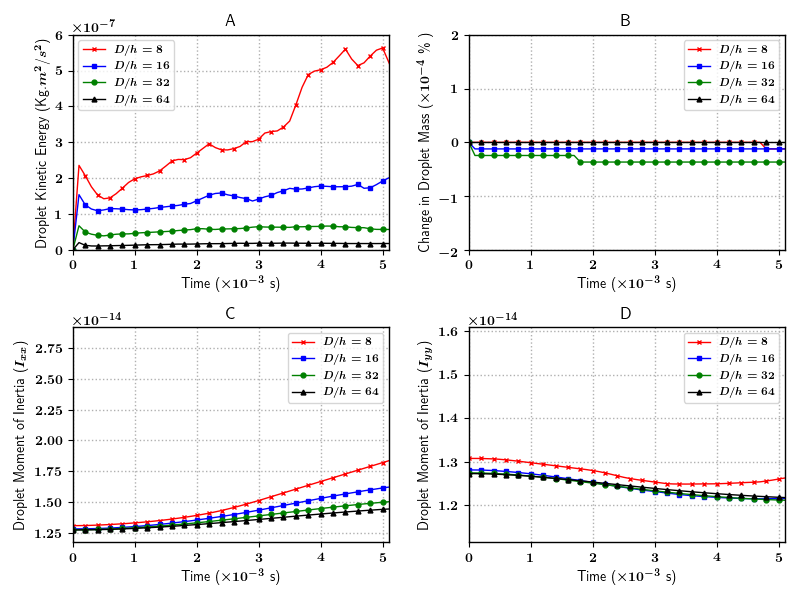
\includegraphics[scale = 0.6]{Figures/Sagar/multiplot_raindrop.png}
\end{center}
\vspace*{-0.5cm}
	\caption{Temporal evolution of quantities of interest to evaluate the performance of our present method for different spatial resolutions. (A) Kinetic energy of the droplet. (B) Percentage change in the droplet mass from initialized mass. (C) Moment of inertia of the droplet along flow (X) direction. (D) Moment of inertia of the droplet along direction perpendicular to flow (Y,Z), evolution of $I_{yy}$ is identical to $I_{zz}$, thus the latter is not shown.}
\label{multi}
\end{figure}

We illustrate the performance of the present method through the results of our simulations in Figure \ref{multi}. The spatial resolutions correspond to $D/h = 8, 16, 32 $ and $64$ using the WY advection scheme in combination with the QUICK flux limiter, while keeping the same value for the inflow velocity boundary condition. The quantities of interest while examining the robustness of the method are the temporal evolution of the droplet kinetic energy (Fig. \ref{multi}. A) and droplet mass (Fig. \ref{multi}. B), as well as moment of inertia of the droplet along directions aligned to the inflow velocity (Fig. \ref{multi}. C) and orthogonal (Fig. \ref{multi}. D) to it. The moment of inertia is used as a descriptor of the 'average' droplet shape, with the three moments of inertia along the different axes $I_m$ defined as - 

\be
I_m = \int_\DDD H x_m^2 {\rm d}\X \;, \quad  1 \le m \le 3,
\nd

where $\DDD$ is the computational domain and $x_m$ is the distance of the interface relative to the center of mass of the droplet.   

\begin{figure}[h!]
\begin{center}
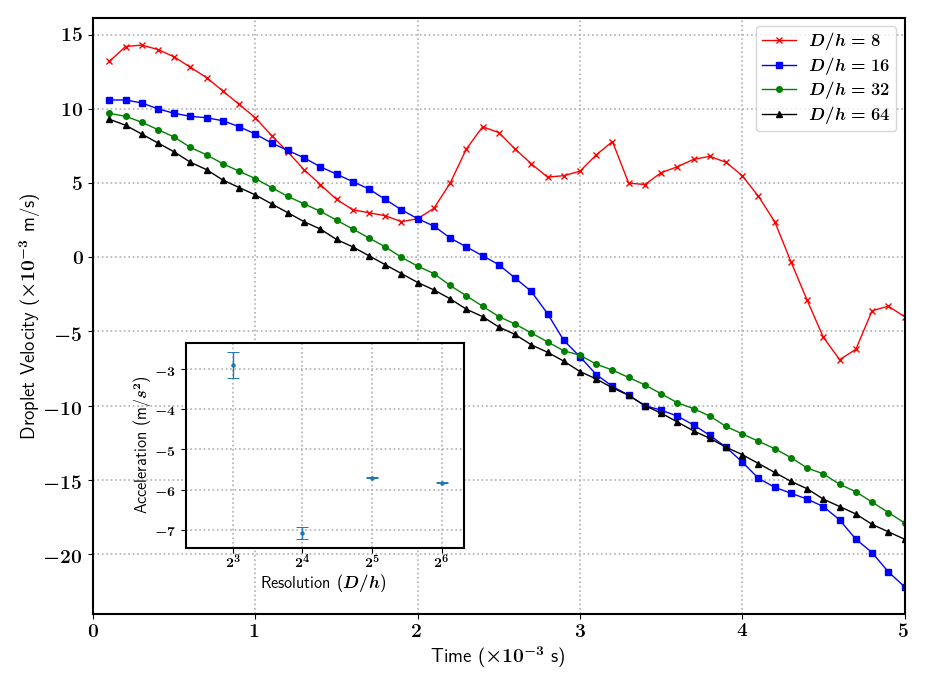
\includegraphics[scale = 0.5]{Figures/Sagar/dropl_velocity_accel_ppd.png}
\end{center}
\vspace*{-0.5cm}
\caption{Comparison of droplet velocity as a function of time, for different droplet resolutions, The droplet velocities correspond to that of their respective center of masses. Inset : Convergence of the droplet acceleration as a function of resolution, computed using the best linear fit over the temporal variation of their respective velocities. The error bars signify the asymptotic standard error (least-squares) corresponding to the obtained linear fits.} 
\label{drop_vel}
\end{figure}

\begin{table}[h!]
\begin{center}
	\hspace*{-0.7cm}
\begin{tabular}{|c|c|c|c|c|}
\hline
Resolution ($D/h$) & $8$ & $16$ & $32$ & $64$ \\
\hline
Acceleration ($m/s^2$) & $-2.89 \pm 11.09\%$ & $-7.08 \pm 1.97\%$ & $-5.70 \pm 0.42\%$ & $-5.82 \pm 0.12\%$ \\ 
\hline
\end{tabular}
\caption{Droplet acceleration in the frame of reference of the static box. The reduction in the error as we increase spatial resolution follows a rate of convergence roughly equal to $2.5$.  \label{acc_err}}
\end{center}
\end{table}

The kinetic energy of the droplet evolves in a relatively smooth manner, without the presence of sudden spikes and falls which are emblematic of the non-conservative version of our method. Such abrupt changes in kinetic energy of the droplet have been found to be associated with instants when the droplet undergoes 'artificial' atomization or breakup, henceforth resulting in the catastrophic loss of stability for the numerical method. We observe a systematic drop in the amount of the droplet kinetic energy as we increase resolution, with the most probable explanation being that of the suppression of spurious interfacial oscillations which are rampant at low resolutions. There is also a component of the kinetic energy of the droplet associated with the internal coherent vortical structures generated due to the interaction of aerodynamic shear at the interface, evidenced by the non-zero value of the kinetic energy even for the most highly resolved droplets. In terms of mass conservation, our method performs well, with the fractional loss of mass bounded within $0.0001 \%$ for all droplet resolutions tested. Finally, the moment of inertia of the droplet appears to evolve in a smooth manner for all droplet resolutions, with higher resolutions exhibiting lower amounts of inertia as a result of the more compact shapes obtained once the spurious interfacial deformation modes are subdued.          

% -----

% Section written by Stephane. Not sure whether to keep this in the current context. 

%------------------------------------------------------------------------------------------
%From the values of the moments of inertia, the horizontal and vertical 
%extents of the droplet (respectively $D_r$ and $D_x$) can be found 
%and compared to the values found by the authors of \cite{Reyssat:2007ko}. 
%We find $D_r=3.1 \,mm$ and $D_x=2.6 \,mm$, while ref. \cite{Reyssat:2007ko} 
%concludes that drops are quasi-spherical for an equivalent diameter 
%$D_e \le l_c$ and deformed for $D_e > l_c$, where $l_c =(\sigma/\rho g)^{1/2}$ 
%is the capillary length, $l_c = 2.7 \,mm$ for water. 
%Indeed repeating the simulations for larger drops we find increased 
%flattening as shown on Figure \ref{flatten}. 

%\begin{figure}[h!]
%\begin{center}
%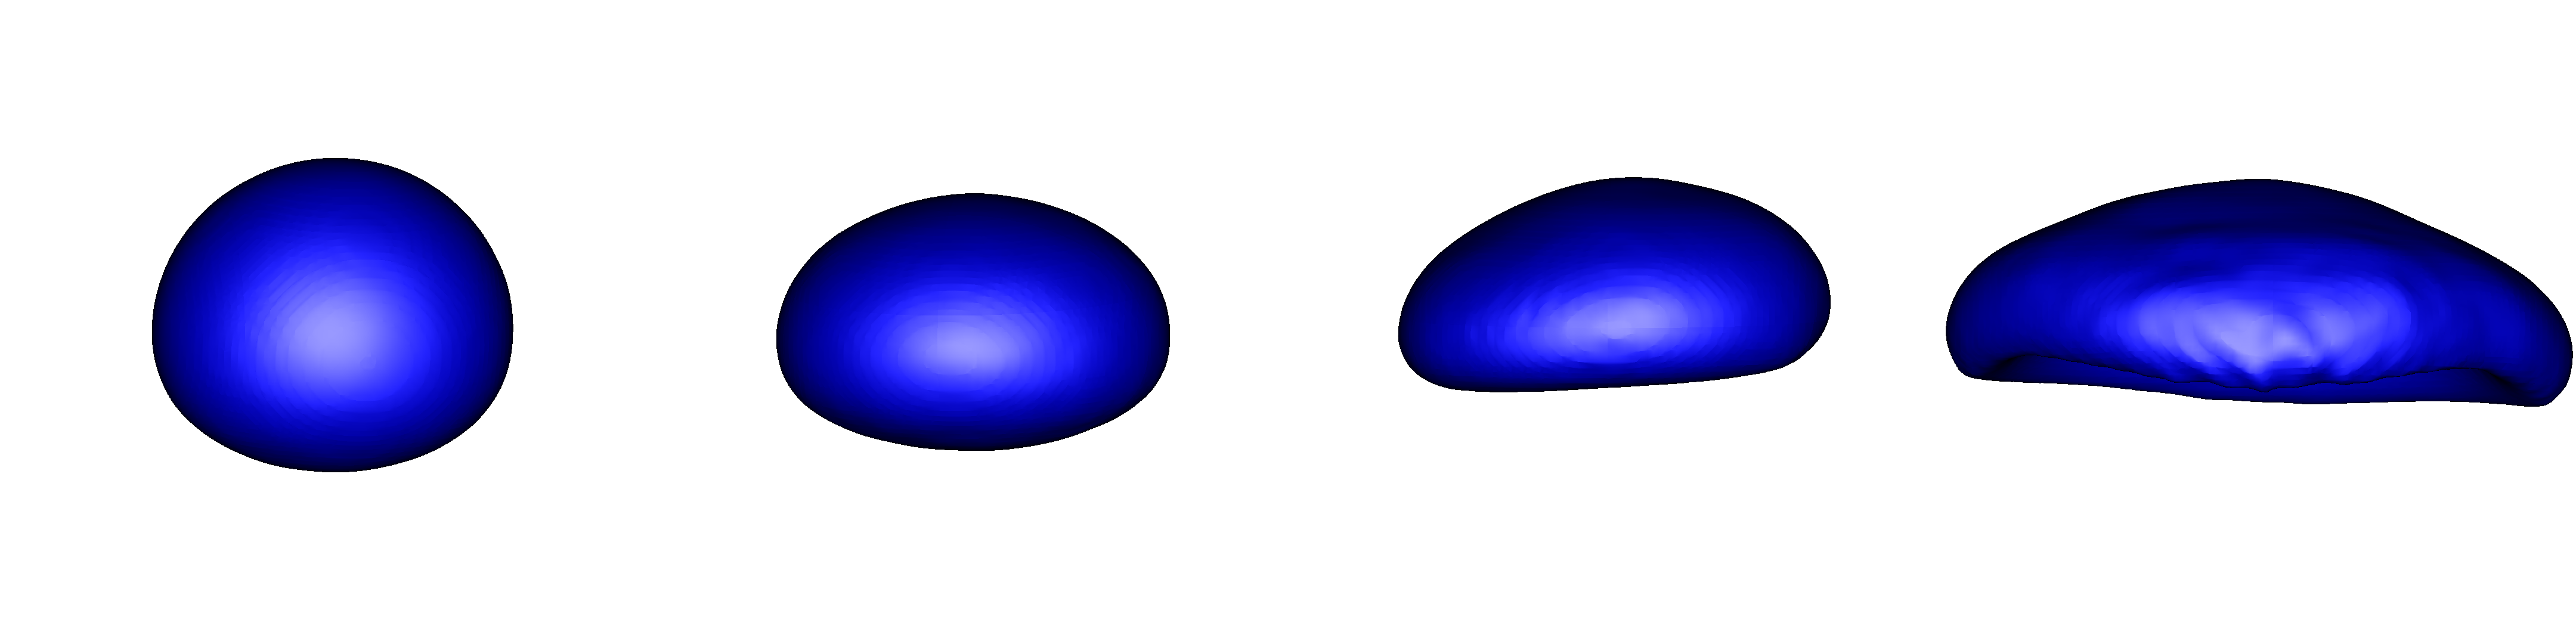
\includegraphics[width=0.99\textwidth]{Figures/flatten.png}
%%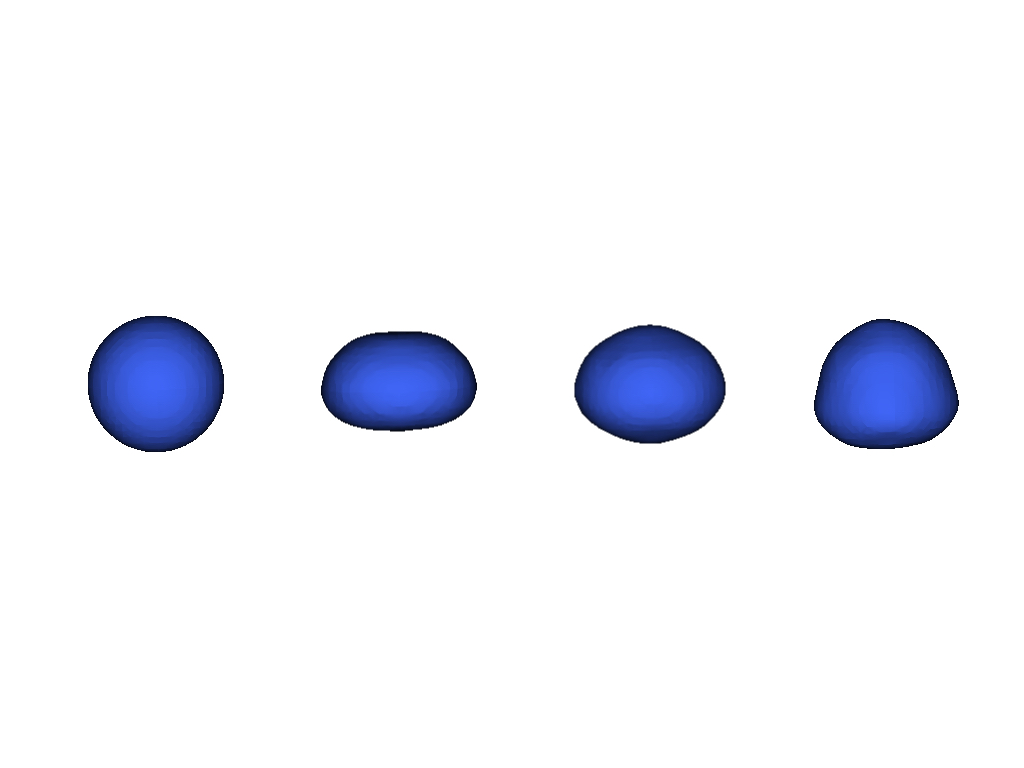
\includegraphics[width=0.99\textwidth]{Figures/Sagar/fig14-001.jpeg}
%\end{center}
%\caption{Flattening of the droplet with increasing equivalent diameter 
%(see text). From left to right $D_e=3, \,4.6,\, 6.4$ and $8\, mm$.}
%\label{flatten}
%\end{figure}
%------------------------------------------------------------------------------------------

\vspace*{0.2cm}


We have to keep in mind that the velocity inflow condition does not correspond to the 'exact' teminal velocity field an actual falling raindrop might experience, hence the droplet in our numerical setup does have some finite acceleration due to the imbalance between the aerodynamic forces and gravity. In Figure \ref{drop_vel}, we demonstrate the velocity of the center of mass of the droplet (in the frame of reference of the box enclosing the droplet) as a function of time, and its behavior as we increase the droplet resolution. As one can observe, due to the imbalance of forces acting on the droplet, it undergoes a net acceleration as evidenced by the approximately linear increase (absolute value) in the velocity as a function of time. The temporal variation in the droplet velocity is fitted to a linear polynomial in order to evaluate the droplet acceleration by means of a standard least-squares approach, for each droplet resolution. We illustrate (inset Figure \ref{drop_vel}) that we achieve more accurate fits as a consequence of higher droplet resolutions, as evidenced by decrease in the standard error on the fits ranging from $\pm 11.1 \%$ for $D/h = 8$ to a value of $\pm 0.12 \%$ for the highest resolution of $D/h = 64$. As per the values given in Table \ref{acc_err}, the reduction in the error as a function of the resolution corresponds to an order of convergence roughly equal to $2.5$ . The results obtained in this section indicate that especially when it comes to low resolutions, our numerical method can be used to get relatively good estimates of the underlying flow features of the droplet without observing an un-physical evolution as a consequence of discretization errors.           


%
%\clearpage

% Slightly less stable methods result when one takes $\hat x = x_i$. 
% In that case we observe at low resolution ($D/h=15$) the energy spike shown 
% in Figure \ref{lowres}. The energy spike is 
% associated with a moving bump on the droplet. Using a higher resolution 
% of $D/h=30$ makes the energy spike disappear. 
% Switching to the shifting of the interpolation point $\hat x$ described in 
% Section \ref{tunedinter}, even more stable behavior is observed, down 
% to resolutions of $D/h=8$. 
% -----
% \begin{figure}
% \begin{center}
% \begin{tabular}{cc}
% 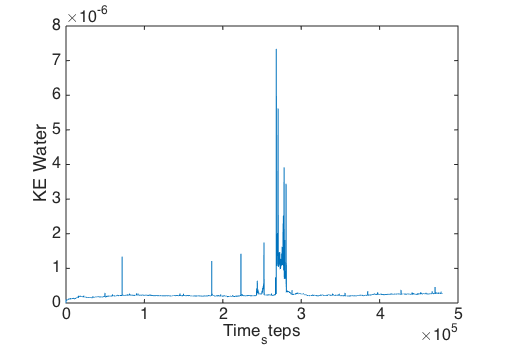
\includegraphics[width=0.5\textwidth]{Figures/KE.png}
% & 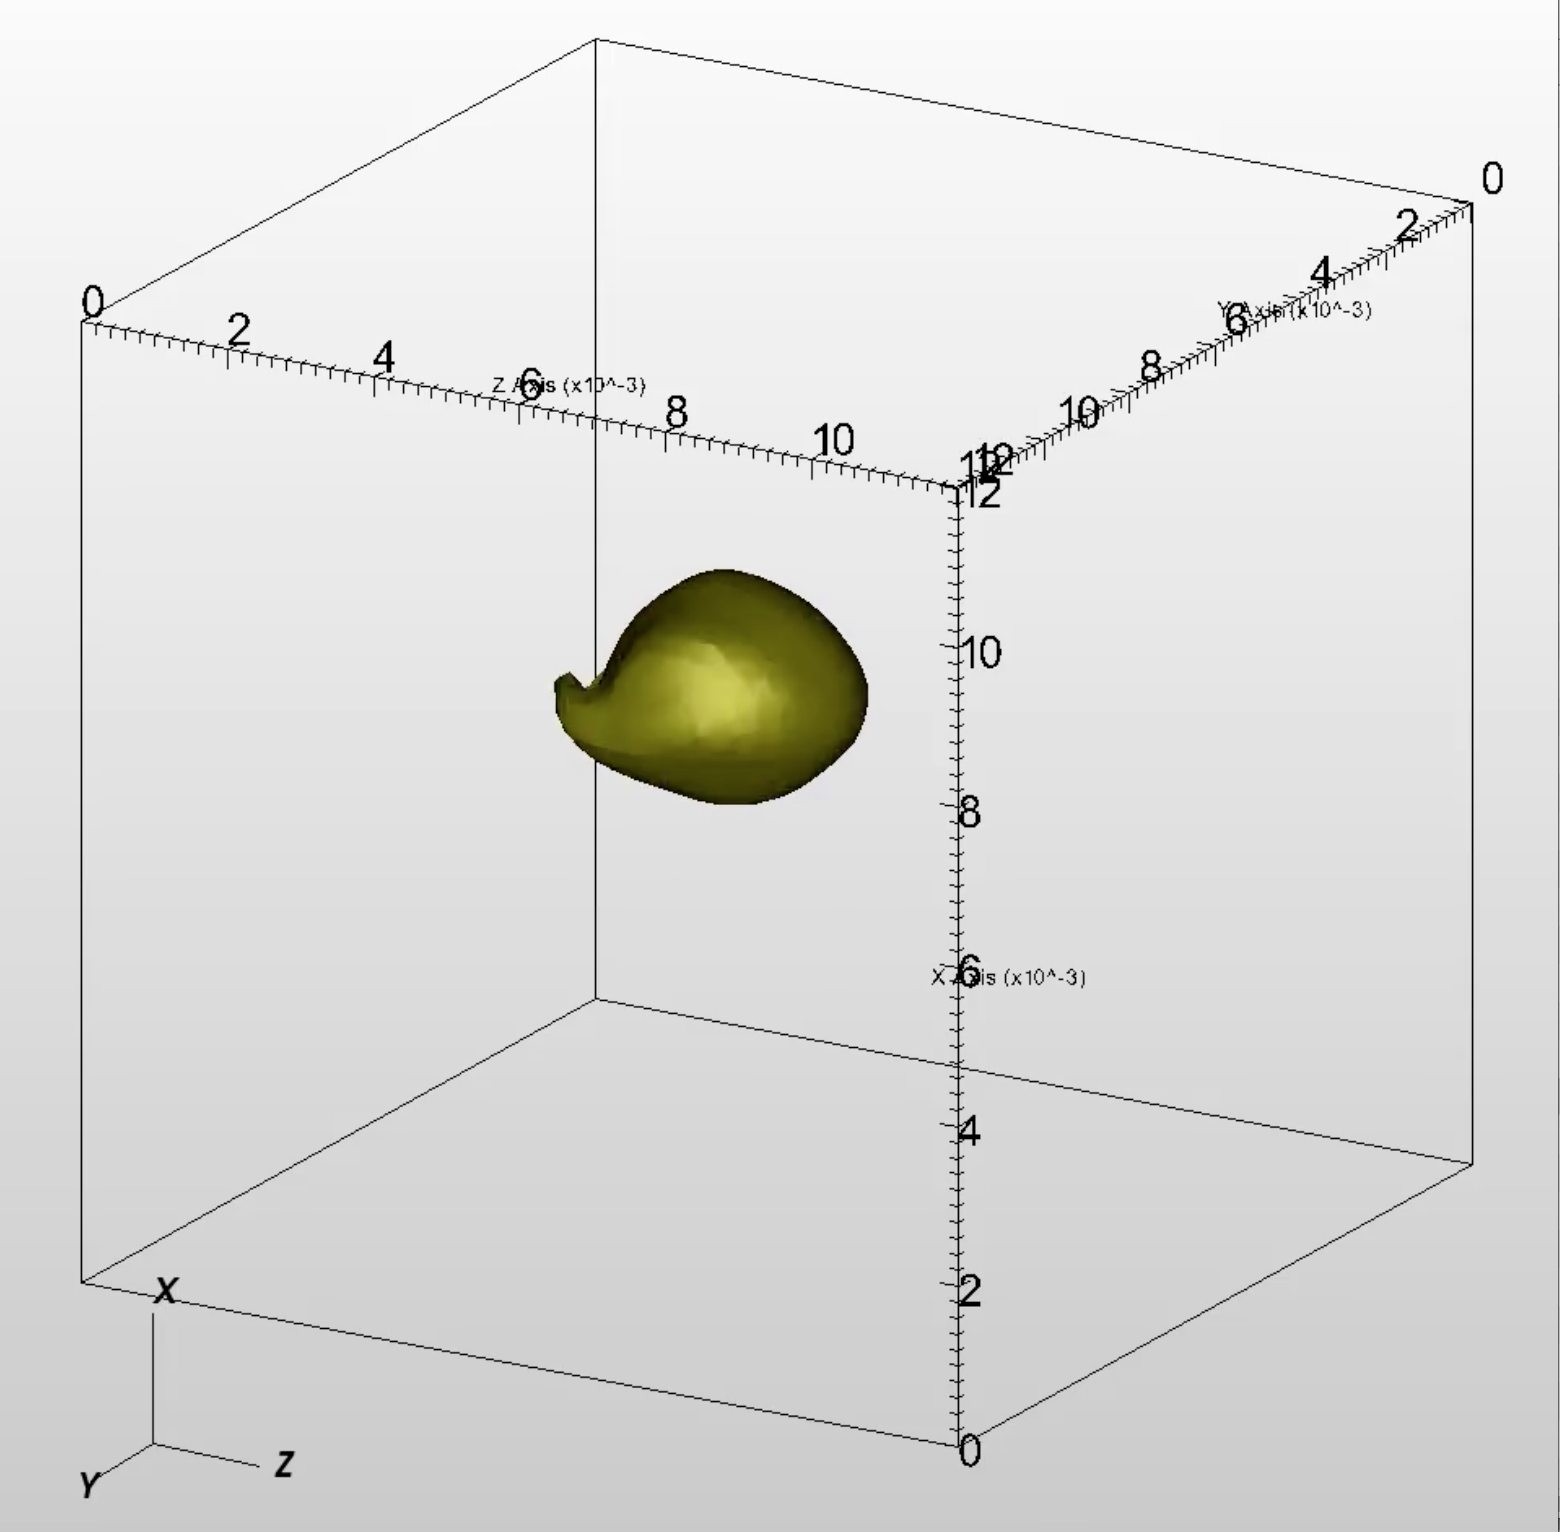
\includegraphics[width=0.4\textwidth]{Figures/bump.png} \\
% (a) & (b)
% \end{tabular}
% \end{center}
% \caption{Effect of a slightly unstable setup. (a) The kinetic energy 
% as a function of time exhibits several
% spikes (b) A snapshot of the simulation at the instant of the formation 
% of the first spike. A pointed
% bump forms on the droplet and starts rotating rapidly.}
% \label{lowres}
% \end{figure}
% -----
%% -----
%\begin{figure}
%\begin{center}
%\begin{tabular}{cc}
%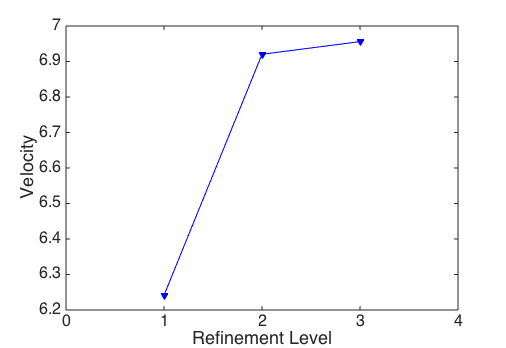
\includegraphics[width=0.45\textwidth]{Figures/veloconv.png}
%& 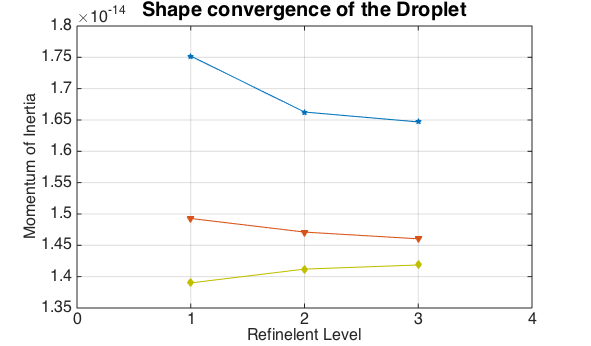
\includegraphics[width=0.45\textwidth]{Figures/shapeconv.png} \\
%(a) & (b)
%\end{tabular}
%\end{center}
%\caption{Convergence of simulations. (a) Evolution of the terminal velocity 
%with grid refinement. (b) Evolution of the three moments of inertia with 
%grid refinement.}
%\label{converge}
%\end{figure}
%% -----
% -----

